%%%%%%%%%%%%%%%%%%%%%%%%%%%%%%%%%%%%%%%%%%%%%%%%%%%%%%%%%%%%%%%%%%%%%%%
%%%                           System Description
%%%%%%%%%%%%%%%%%%%%%%%%%%%%%%%%%%%%%%%%%%%%%%%%%%%%%%%%%%%%%%%%%%%%%%





\chapter{System Description}

This chapter will discuss our game design, the story, mechanics, and tools used, and briefly discuss the previous iteration.

\section{Game Description}
The game is developed on React\footnote{\url{https://reactjs.org/}} with Chakra UI\footnote{\url{https://chakra-ui.com}}. We use Supabase\footnote{\url{https://supabase.com/}} to keep logs of user interaction with the game. Figure \ref{fig:screenshot} shows the initial state of the game.

\begin{figure}[h]
    \centering
    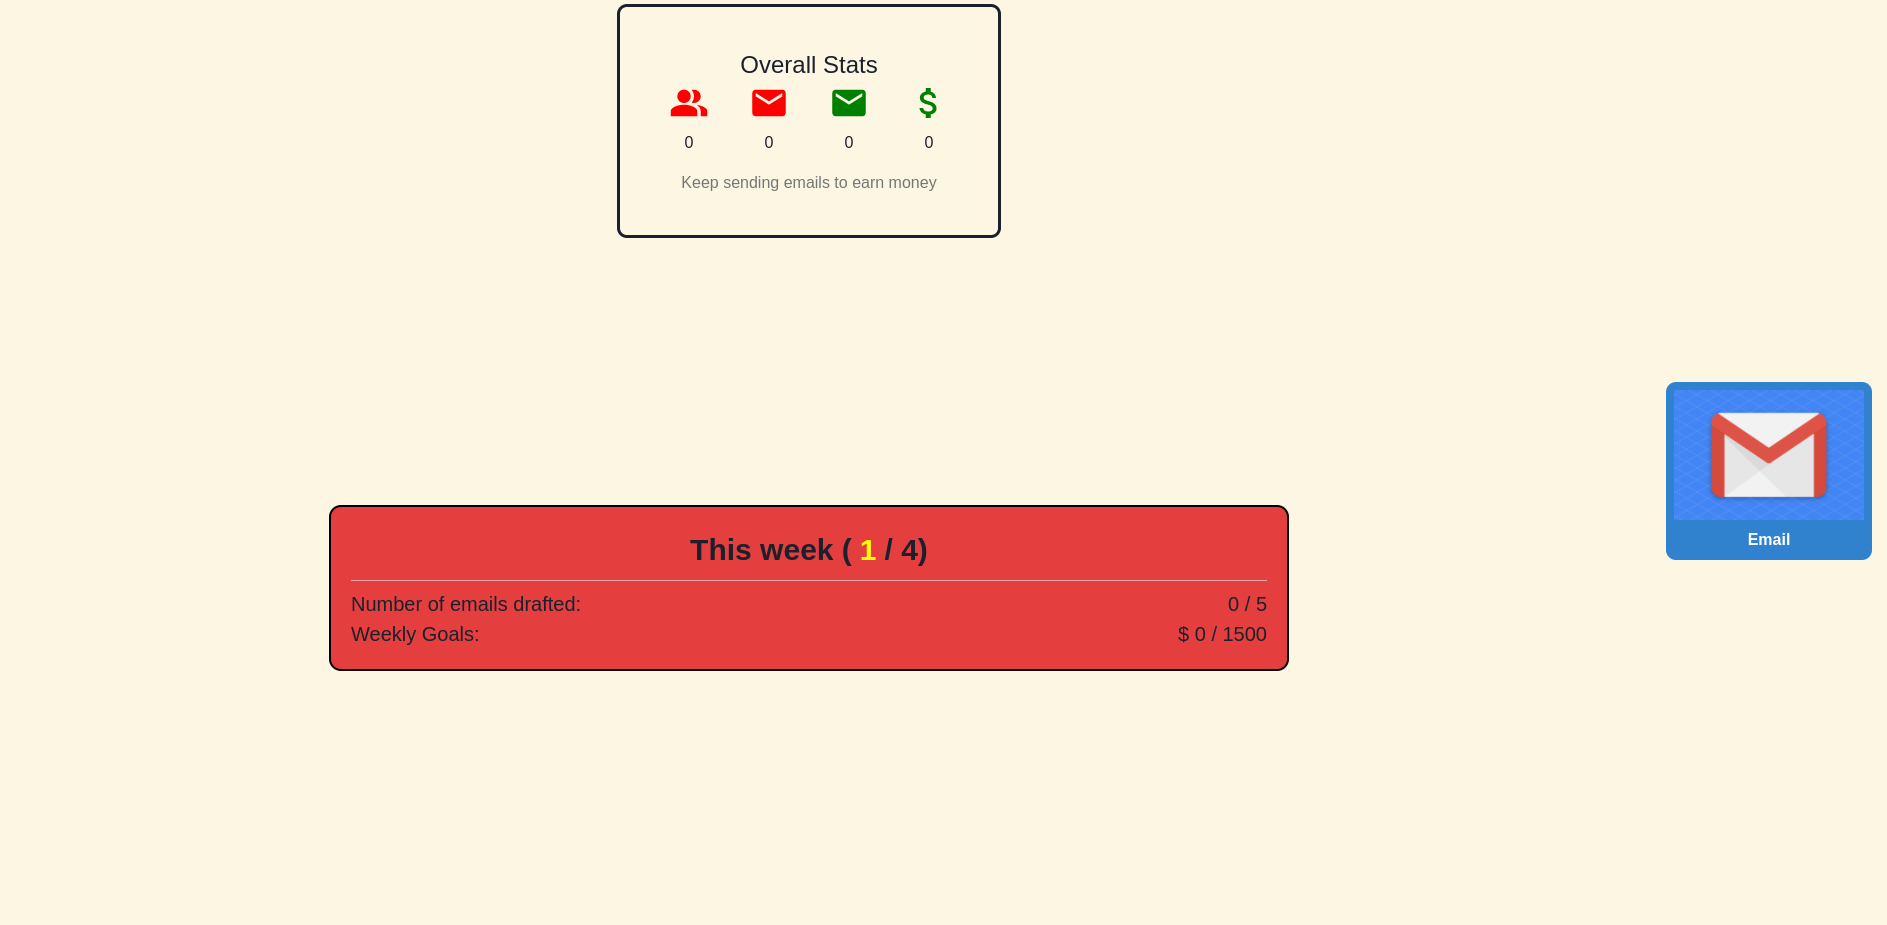
\includegraphics[width=\textwidth]{figures/section2/game.png}
    \caption{Screenshot of initial state of the game}
    \label{fig:screenshot}
\end{figure}

\subsection{Game Story}
The game's main character has taken a large loan from a loan shark. The goal of the game is to pay off the loan in time. However, as the loan is substantial, he cannot earn enough money through hard work and uses phishing tricks to scam people. However, the main character does not have enough skills, so he hires a helper to create phishing emails. Together, they have decided to impersonate PayPal. The player has four weeks to earn enough money to pay back.

\section{Mechanics}
One of our main objectives while developing the game was to streamline the player experience. We divided the game into four weeks (parts) to achieve this goal. Each week's progression will unlock specific skills users' can use to create an email. We will discuss specific week progression and how it ties the game together in later sections.

\subsection{Components}
Before we deep dive into the game's flow, we have to discuss individual components. At the top level, we can divide the game into three components: attacker, marketplace, and email generation.

\subsubsection{Atttacker}
The attacker module handles training the helper with available skills. There are six different skills that the player can train the helper on, namely spelling, grammar, styling, links, spoofing, and research. We divide these skills as language skills (spelling and grammar) and technical skills (styling, links, spoofing, research). Language skills are passive skills in the game, whereas technical skills, except for styling, are active skills.

Training on passive skills will improve the quality of the email generated by the helper without any additional input from the player. In contrast, active skills will give the player more options while generating the email. For example, after the player trains their helper on spelling, the attacker will stop making spelling errors without additional feedback from the user. Training the helper on links will give the user different options to hide the links while creating the email. Table \ref{tab: attacker} lists the skills and their effect in the game in brief. We will talk about the different properties activated by each skill in the email generation section.

\begin{table}[!ht]
    \centering
    \resizebox{\textwidth}{!}{%
        \begin{tabular}{p{0.05\textwidth} p{0.05\textwidth}  p{0.05\textwidth}  p{0.5\textwidth}}
            \hline
            \textbf{Skills} & \textbf{Active/} & \textbf{Cost} & \textbf{Effect}                                                   \\
                            & \textbf{Passive} &               &                                                                   \\
            \hline
            Spelling        & Passive          & 1,000         & Creates emails without spelling errors                            \\
            Grammar         & Passive          & 1,000         & Create emails without grammar errors                              \\
            Styling         & Passive          & 2,000         & Create stylized emails with better header, footer, and images     \\
            Links           & Active           & 3,000         & Unlocks different techniques to hide the link while sending email \\
            Research        & Active           & 3,000         & Gives the user option to generated targeted emails                \\
            Spoofing        & Active           & 4,000         & Gives the user ability to spoof the email                         \\
            \hline
        \end{tabular}%
    }
    \caption{Different skills and their effect in the game}
    \label{tab: attacker}
\end{table}

We chose the skills in the game to replicate the training objective of existing training modules and common properties found in phishing emails. Each skill in the game has a training cost associated with it. We associated some costs with skills to represent training requires some resources. The cost is kept at a minimum to let the user unlock it as soon as possible but scaled such that more efficient skills have a higher price than general skills. Keeping the cost low allowed the user to focus more on using those skills to generate emails rather than earning money to train attackers.

\begin{figure}[!ht]
    \centering
    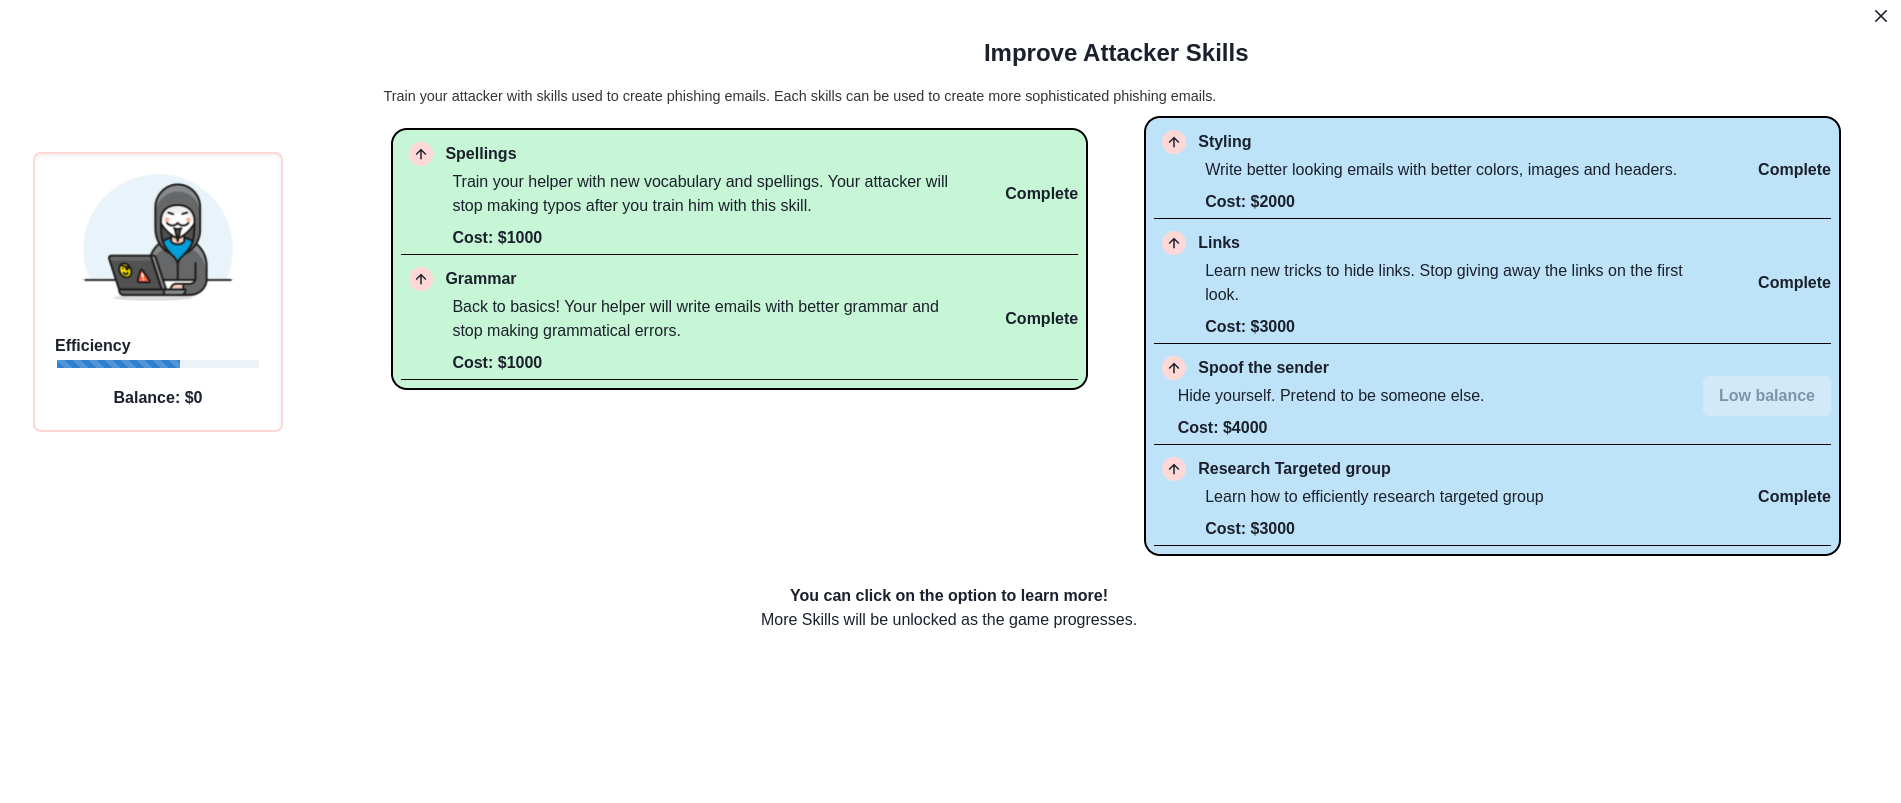
\includegraphics[width=\textwidth]{figures/section2/attacker.png}
    \caption{Screenshot of the attacker module on week 4}
    \label{fig:attacker}
\end{figure}

Although we tried to include all the common properties found in phishing emails, we could not itemize some general properties such as sense of urgency, generic greetings, too good to be true emails, et cetera. Instead of itemizing and adding more passive skills, we decided to limit the number of skills and let users actively concentrate on those. On the technical side, the limited number of properties to look at while generating emails made email generation much more manageable and allowed us to generate a broader range of emails. Current emails generated by the system still include the properties of phishing emails that we could not itemize. Exposing players to more phishing emails may help players recognize similar emails and patterns later.

\subsubsection{Marketplace}
The marketplace allows the player to purchase domains to use while generating emails (See figure \ref{fig:marketplace}). Existing training modules train the players to recognize phishing links (which are generated by the system) but do not allow players to try custom domains. In our gameplay, the attacker "link" skill teaches how phishing emails hide links to trick victims into clicking the link.

\begin{figure}[!ht]
    \centering
    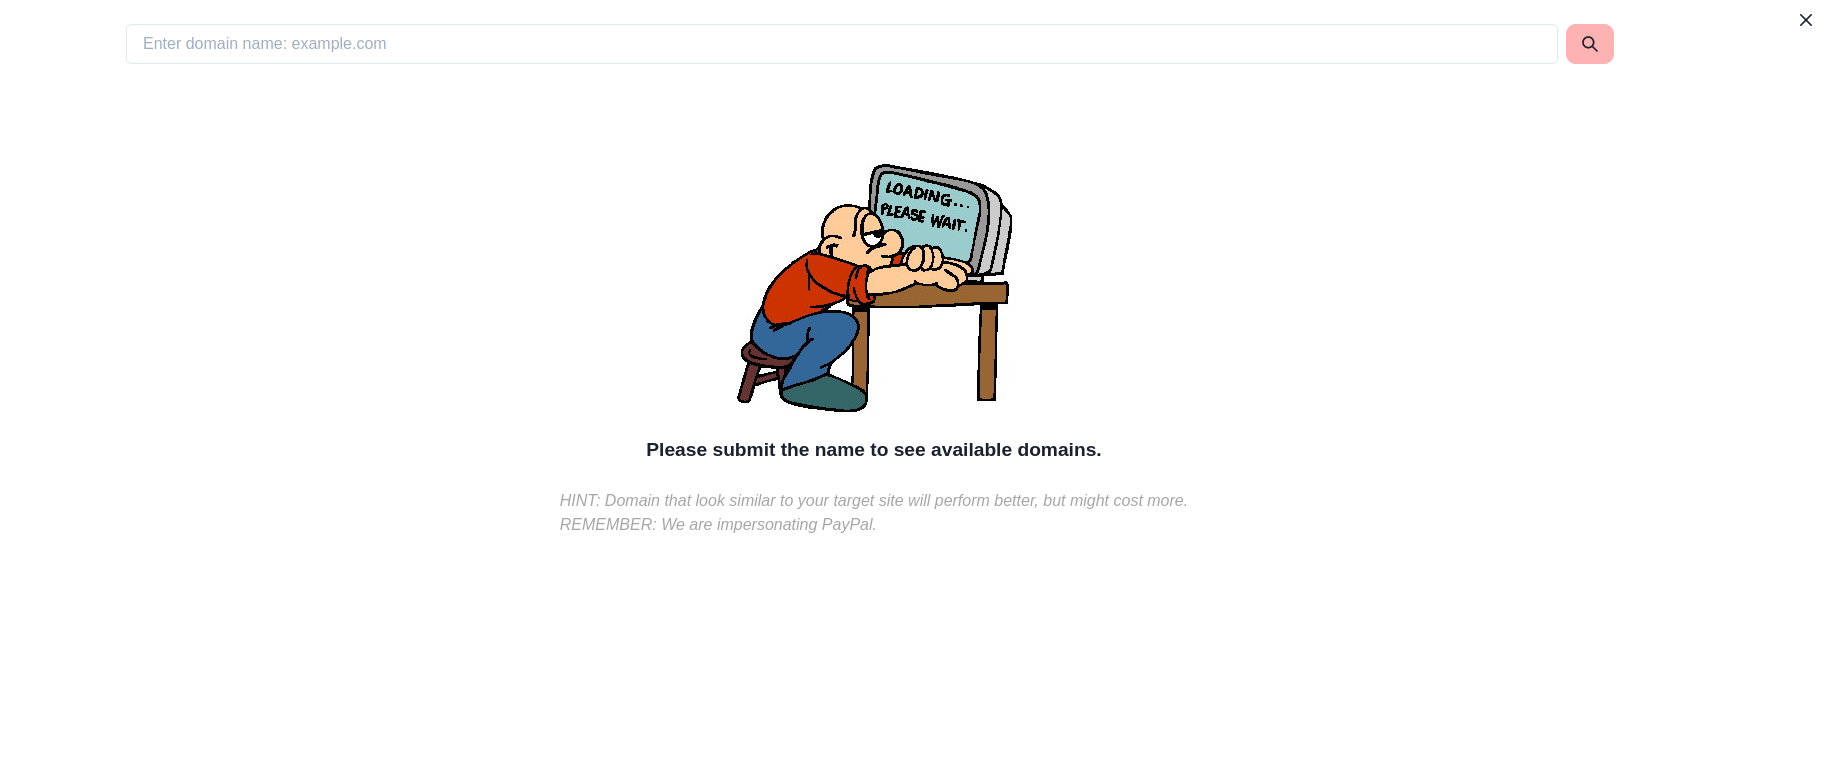
\includegraphics[width=1\textwidth]{figures/section2/marketplace_empty.png}
    \caption[Screenshot of marketplace]{The marketplace accepts any valid domain name}
    \label{fig:marketplace}
\end{figure}

The first step when letting the user purchase a domain is to check if the domain is valid. A valid domain is a second-level domain followed by a top-level domain in our game. A top-level domain refers to the last segment of a domain name, and a second-level domain refers to the name just to the left of the top-level domain. For example, "test.com" is a valid domain where "test" is a second-level domain and "com" is the top-level domain. We validate the second-level domain with the help of the following regex code:

\begin{lstlisting}
    if (userLink.includes(" ") || !/^[a-zA-Z0-9-.]*$/.test(userLink))
        return;
\end{lstlisting}

We do not allow special characters (Fada Accent) in the domain name for simplicity.

There are 1,500 top-level domain \cite{tld}. For simplicity, we only allow users to choose from a predefined list filtered from Tranco list \cite{trancos}. Tranco list provides us with the most popular one million domains, similar to Alexa top site. We filtered top-level domains that occurred a hundred times from Tranco's list and got 262 top-level domains. This limited number of top-level domains allowed us to incorporate commonly used domains while maintaining the game's simplicity.

\begin{figure}[h]
    \centering
    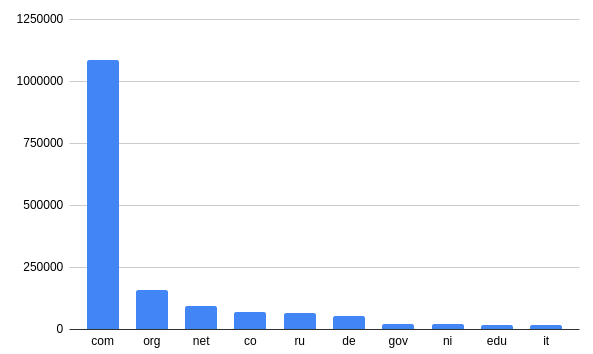
\includegraphics[width=0.7\textwidth]{figures/section2/tld.png}
    \caption{Top 10 top level domains present Tranco list}
    \label{fig:marketplace_tld}
\end{figure}

Players can choose any combination of valid characters for the second-level domain (validated by the regex pattern shown above). For example, "123test.com" is a valid domain. However, "\%ssda1.com" is not a valid domain. We maintain the top 1000 domains in the Tranco list to prevent purchasing popular and already existing domains. This list consists of popular sites such as "google.com," "facebook.com," "netflix.com," including "paypal.com" (which is used by our game to train the user). We had to trim the number of domains to a thousand as processing a million domains required significant processing time, impacting the gameplay.

Our game uses PayPal to trick the victims, so domains closer to PayPal will perform better. Similar to the real world, purchasing a new domain requires money. Domains similar to popular services (determined in the top 1000 domains) will have a higher cost. Since the user can purchase any domain and domain closer to the top thousand domains are more expensive,  the cost of a domain purchased does not directly correlate to higher efficiency in the game.

We determine the closeness between two domains based on string similarity. We use Sørensen-Dice coefficient to compute the similarity between two strings. Mathematically, given two sets, X and Y, we can define Dice coefficient as:

\begin{center}
    \begin{math}
        DSC = \frac{2|X \cap Y|}{|X|+|Y|}
    \end{math}
\end{center}

It produces a value between zero and one, making the cost calculation of domains much easier. Table \ref{tab:dice} shows examples of some custom domains along with their similarity. We can see that a domain similar to "paypal" has a higher similarity. Therefore, we treat domains with higher similarity score as more efficient for our game. We do not use the top-level domain for cost calculation, as most players usually choose ".com," which impacts the string similarity.

\begin{table}[!ht]
    \centering
    \begin{tabular}{r|l}
        \textbf{Custom Domain} & \textbf{Similarity with "paypal"} \\
        \hline
        paypale                & 0.90                              \\
        palpay                 & 0.80                              \\
        paypl                  & 0.66                              \\
        appl                   & 0                                 \\
        test                   & 0                                 \\
    \end{tabular}
    \caption{Different second level domain and their similarity with "paypal"}
    \label{tab:dice}
\end{table}

The cost of the domain does not depend solely on similarity to "paypal". While calculating the cost, we get the maximum similarity with any of the domains in the top-1000 list. If the similarity with the existing domains is below 0.6, we assign a base price of 500 for the domain; else, the general cost of the domain is calculated as:
\begin{center}
    \begin{math}
        cost = 500 + (similarity *100)^2 * 0.56
    \end{math}
\end{center}

If the player tries to buy existing domain, the game suggests domains ending with alternate top level domains (See figure \ref{subfig:marketplace-unavailable}). For example, if the player tries to buy "paypal.com", the game suggests top 10 alternate top level domains such "paypal.org" or "paypal.net". The cost of such domain is not based on similarity. We use the frequency of top level domains in Tranco list and compute the cost as follows:

\begin{center}
    \begin{math}
        cost = (50 * \sqrt{10-index}) *25
    \end{math}
    \text{where index is the ranking of the top level domain based on frequency in Tranco list.}
\end{center}



\begin{figure}[!ht]
    \centering
    \subfloat[Marketplace unavailable\label{subfig:marketplace-unavailable}]{%
        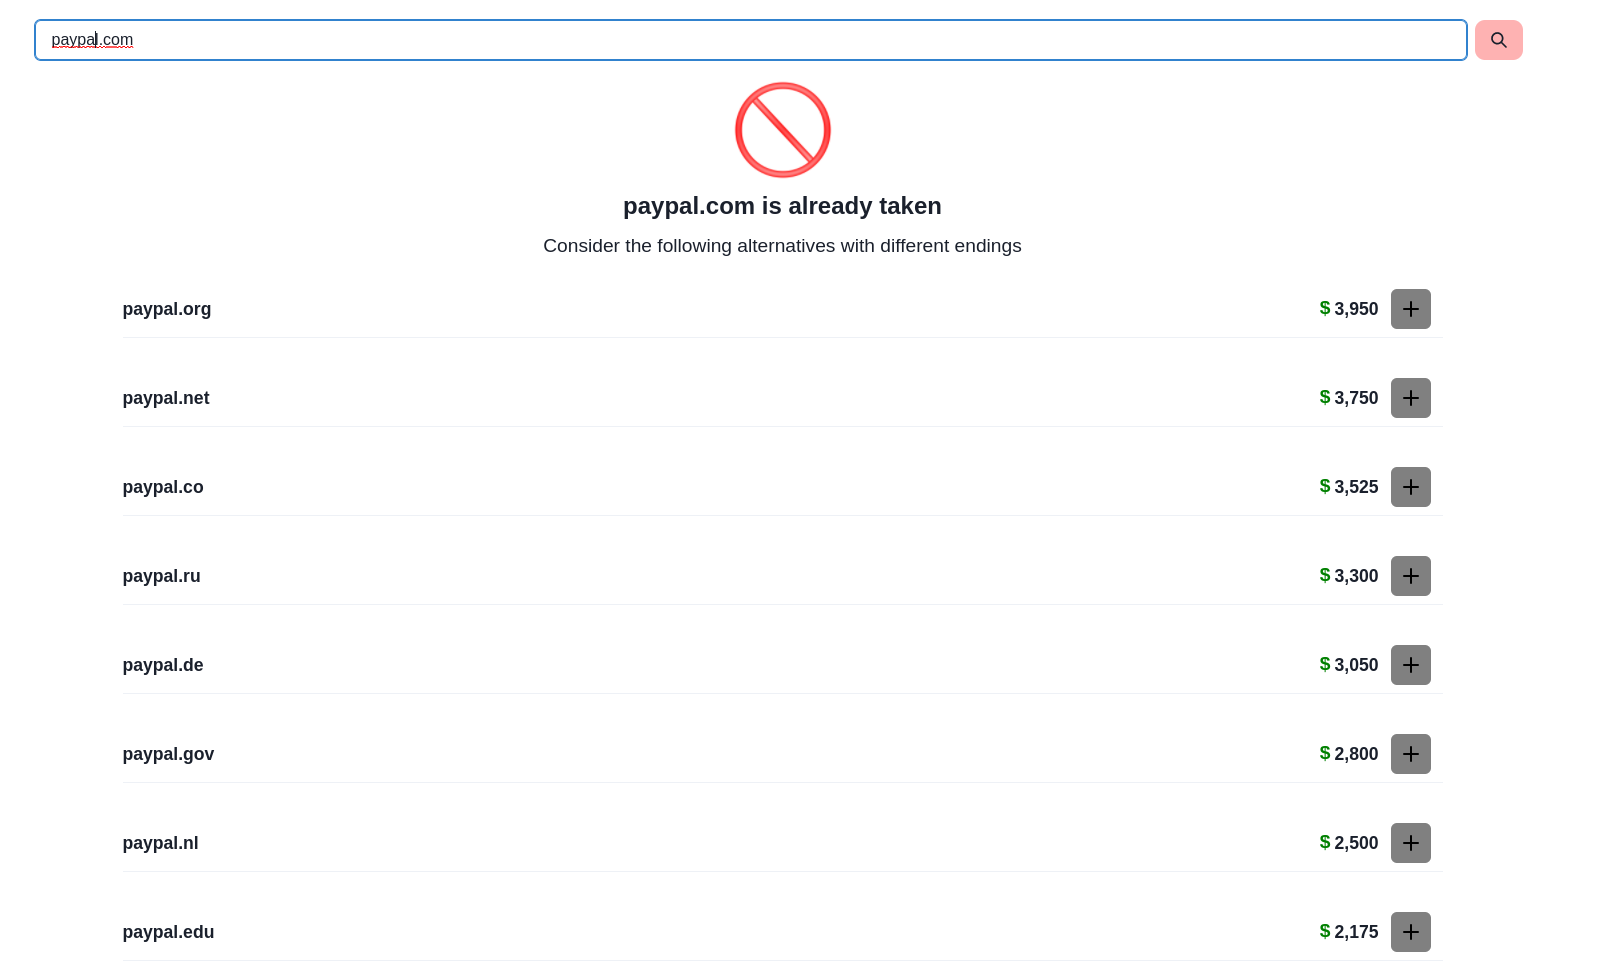
\includegraphics[width=0.9\textwidth]{figures/section2/marketplace_unavailable.png}
    }
    \hfill
    \subfloat[Marketplace available\label{subfig:marketplace-available}]{%
        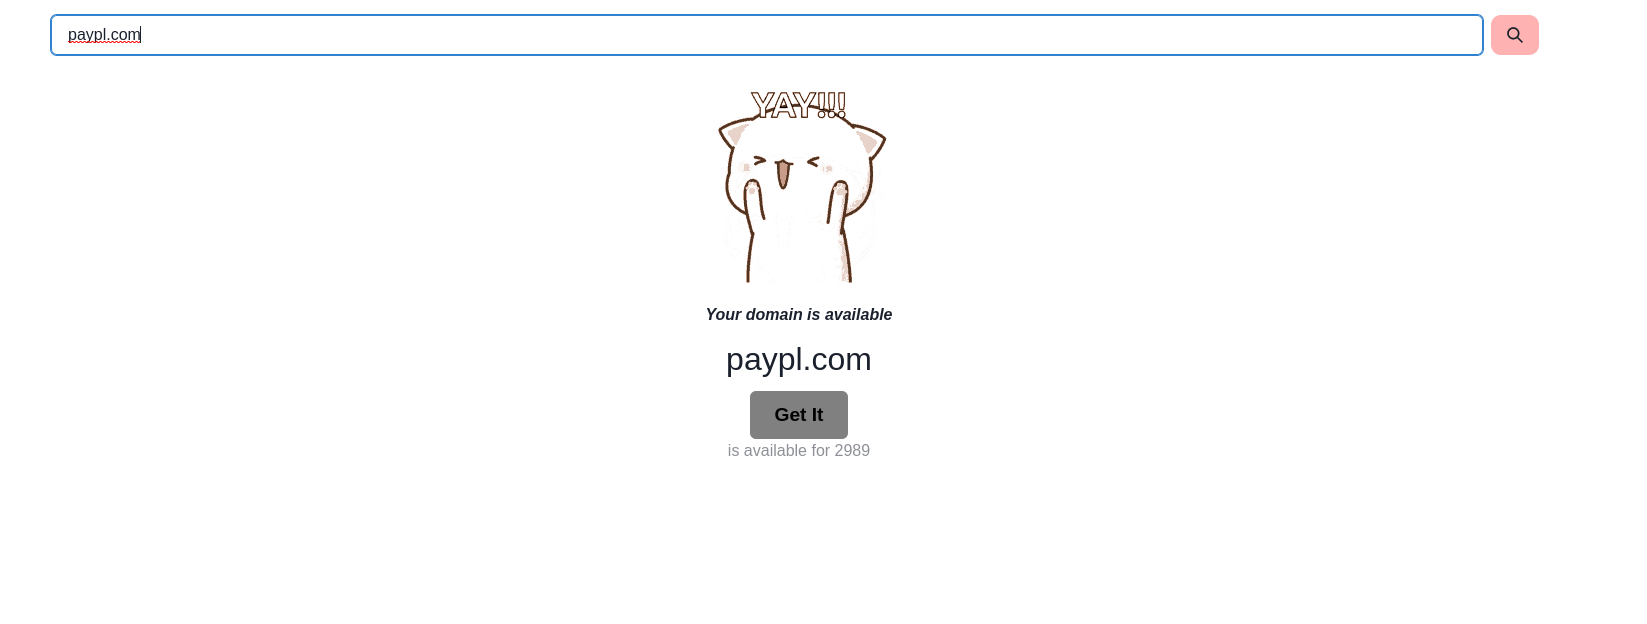
\includegraphics[width=0.45\textwidth]{figures/section2/marketplace_available.png}
    }
    \hfill
    \subfloat[Marketplace invalid\label{subfig:marketplace-invalid}]{%
        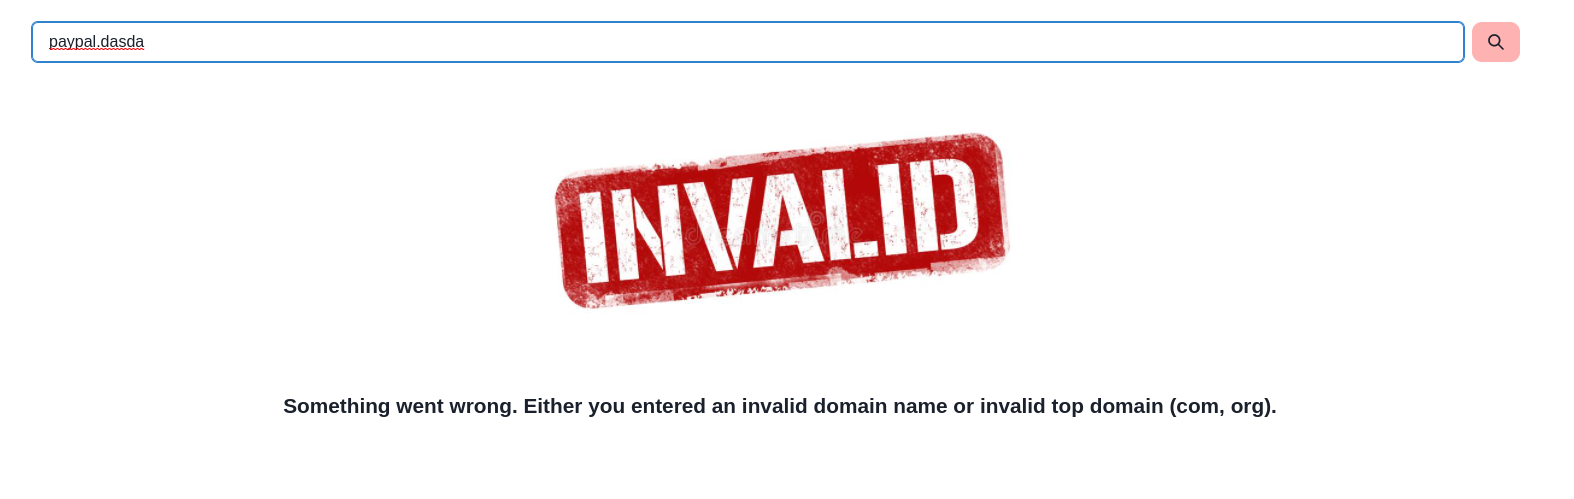
\includegraphics[width=0.45\textwidth]{figures/section2/marketplace_invalid.png}
    }
    \label{fig:marketplace-state}
    \caption{Different stages of the marketplace}
\end{figure}

These formulas to calculate cost are not standard and were achieved through trial and error. Although not an actual scale, we set the cost to show that domains closer to real-world domains will have a higher cost.
% with changes to game, we changed the scale to make it achievable

\subsubsection{Emails}
The emails component ties up the game by generating and sending emails based on attacker skills and the current domain. The system randomly chooses an email from 30 available emails based on the user input (active and passive skills). These emails were handpicked to replicate real-life phishing attempts and include the most commonly found phishing emails. As a result, emails in the system include common phishing tricks used by attackers and different email models such as log-in, welcome emails, limited account emails, et cetera.

Before discussing sending email and efficiency, let us discuss how each skill impacts the email generation process. As mentioned in the attacker component section, passive skill does not require additional input from the player and improves the generated email after training them. Spelling, grammar, and styling in our game fall under passive skills. Before players train on spelling and grammar, they will be required to recognize spelling and grammar errors. We wanted to point out spelling and grammar errors as they are commonly found in poorly worded phishing emails and recognized as one of the common ways to differentiate phishing emails from legitimate emails. However, we do not want users to spend all their time finding language errors, so we generate emails with proper grammar and spelling after training.

Styling increases the visual appeal of the email with the help of images, header, footer, and better styles. Emails sent by an organization generally contain images and styling. Attackers use this fact to trick victims by including company logos and images. As stated before, users generally trust familiar logos and 34\% of users believe emails with familiar logos are safe \cite{proofpoint}.

\begin{figure}[!ht]
    \centering

    \subfloat[Emails generated after training on passive skills generate emails with proper grammar and spelling with styling\label{subfig:passive-trained}]{%
        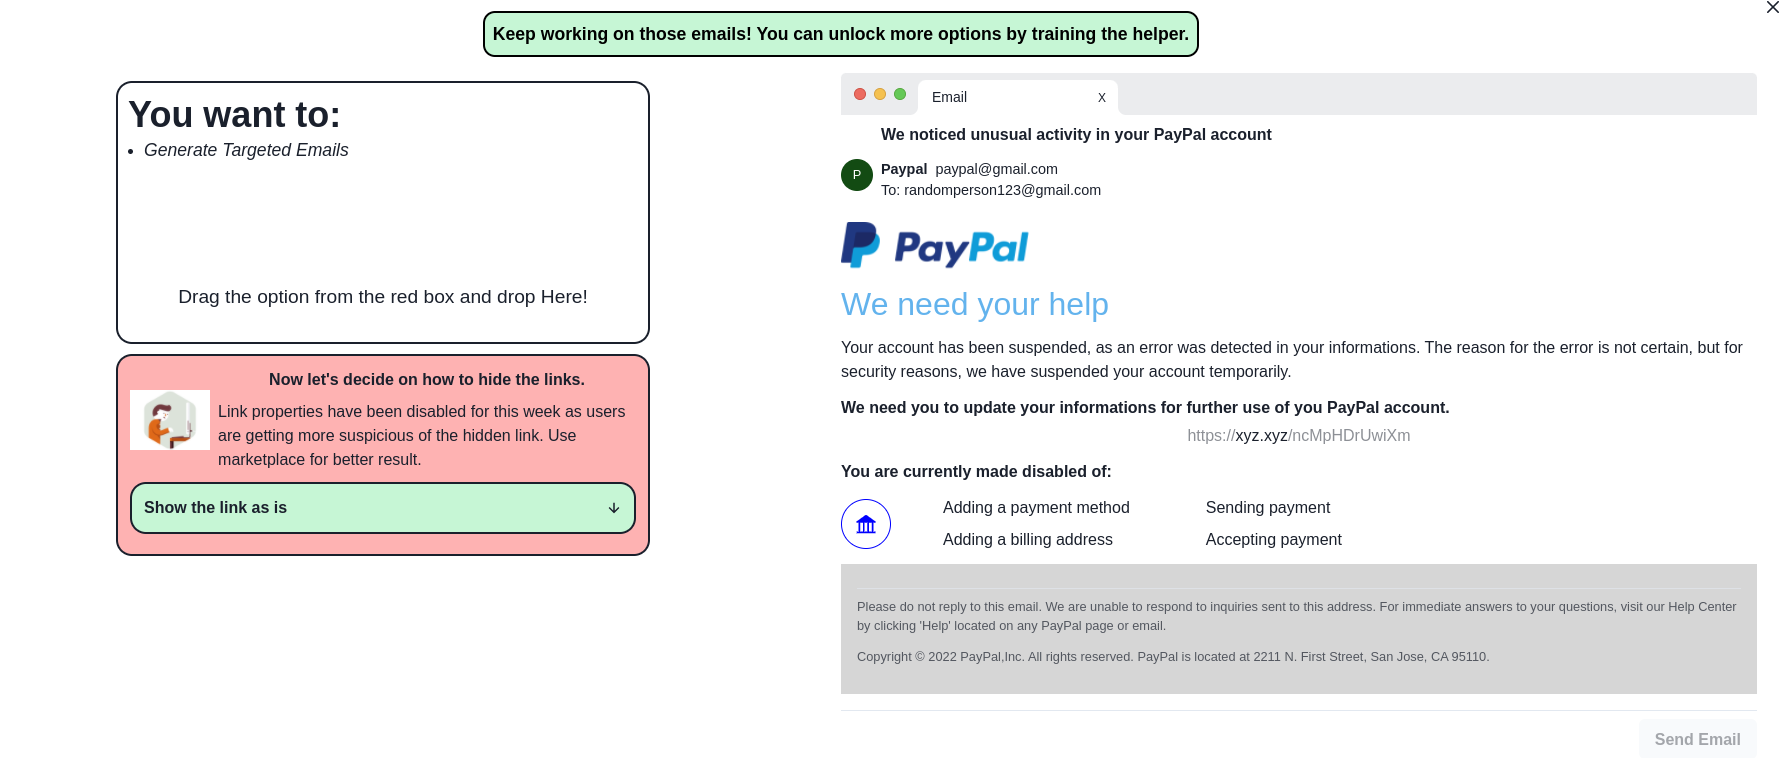
\includegraphics[width=0.75\textwidth]{figures/section2/passive_trained.png}
    }
    \hfill
    \subfloat[Emails generated before training on passive skills contains spelling and grammar error with no styling (contains text only)\label{subfig:passive-untrained}]{%
        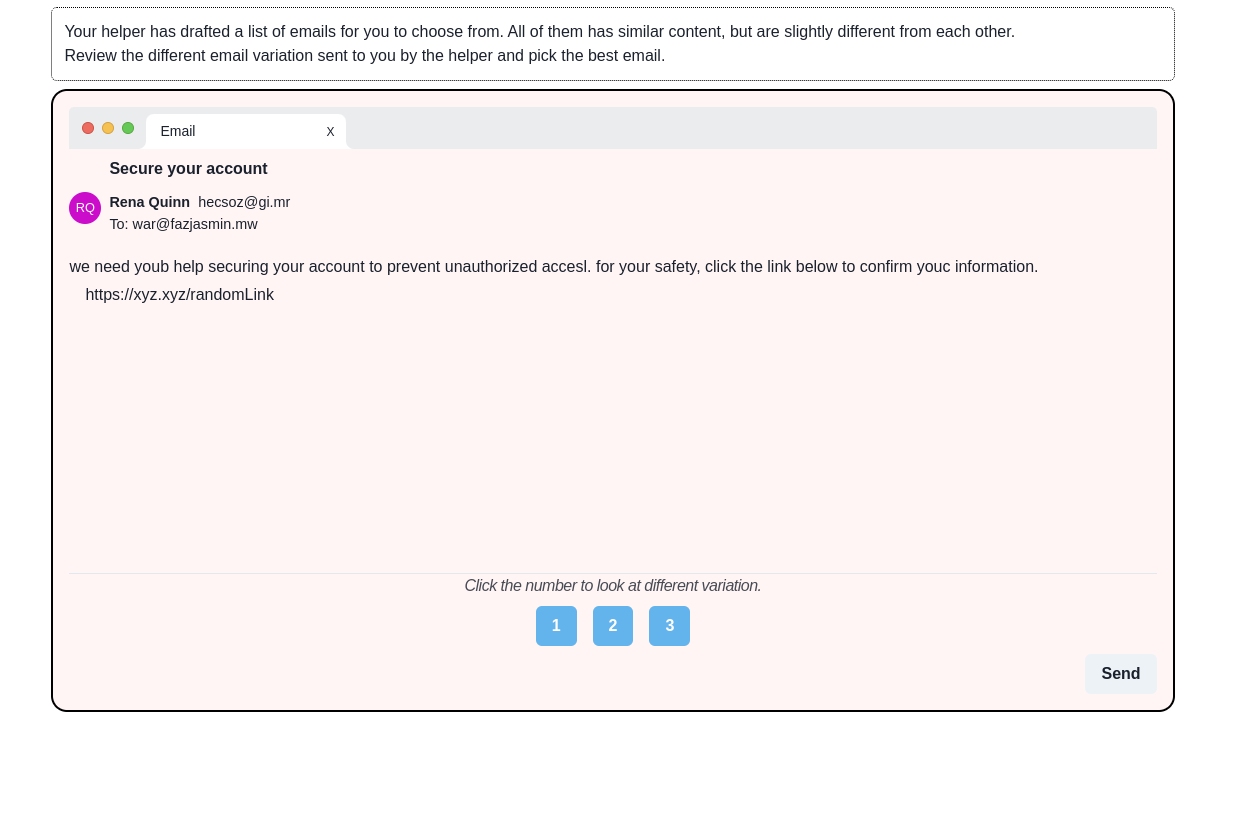
\includegraphics[width=0.75\textwidth]{figures/section2/passive_untrained.png}
    }
    \hfill

    \label{fig:passive}
    \caption{Emails generated after training vs before training on passive skills}
\end{figure}

Active skills give the user more options to fine-tune the generated email. Our game's active skills are links, research, and spoofing. Each option allows the user to modify a part of the generated email. We discuss each of these skills in detail below.

Research skill allows the player to generate targeted emails. Our game approaches the concept of spear-phishing with targeted email. Before training on research, the helper only generates a generic email, and players do not get an option to send targeted emails. Generic emails target a larger audience and do not contain any specific user details. On the other hand, targeted emails contain user-specific information such as address and name.

\begin{figure}[ht]
    \centering
    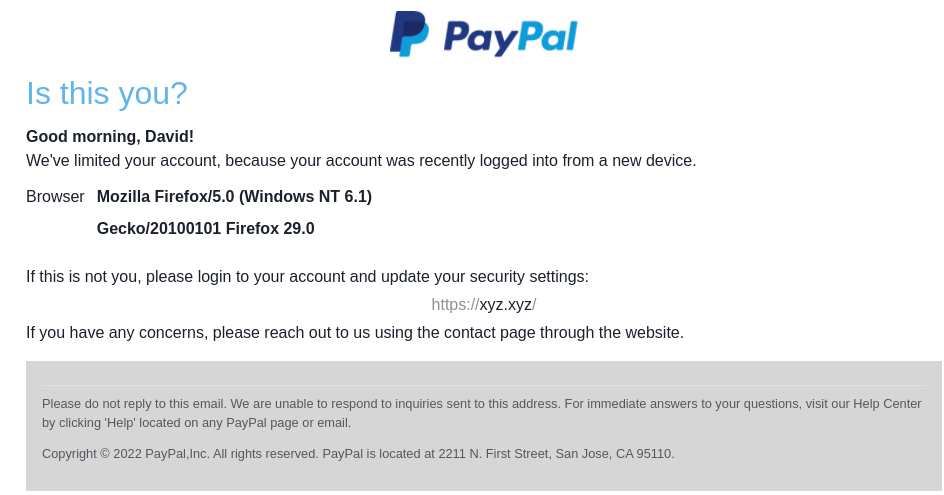
\includegraphics[width=0.9\textwidth]{section2/targeted.png}
    \caption{Example of a targeted email generated by the system}
\end{figure}

All the emails on the system are pre-labeled to either generic or targeted. When the user chooses an option, the system will filter out emails (based on user option) and randomly choose an email from the filtered list.

Our second active skill, links, attempts to cover URL/link training many current phishing training games covers. Training helper on link unlocks different ways to display the link when generating an email. We chose these options after reviewing real-world phishing emails and current training materials.

The game allows the user four different ways to display the link:

\begin{enumerate}
    \item \textbf{Hide under button or text}\\
          One common phishing trick is to hide the actual link behind some text or button. We replicate this behavior with our "Hide link" option, which displays some text or buttons as links without displaying the actual link. To familiarize users with different forms of text messages and buttons, we randomly choose a text message( Example figure \ref{fig:hide-text}) or button (Example figure \ref{fig:hide-button}) from predefined set of input. Our input contains familiar texts such as "Click here," "Go to PayPal," "www.paypal.com/help," and other similar alternatives. Players can hover the text or button to visualize the link (similar to real email clients).

          \begin{figure}[ht]
              \subfloat[The actual link is hidden behind the button]{%
                  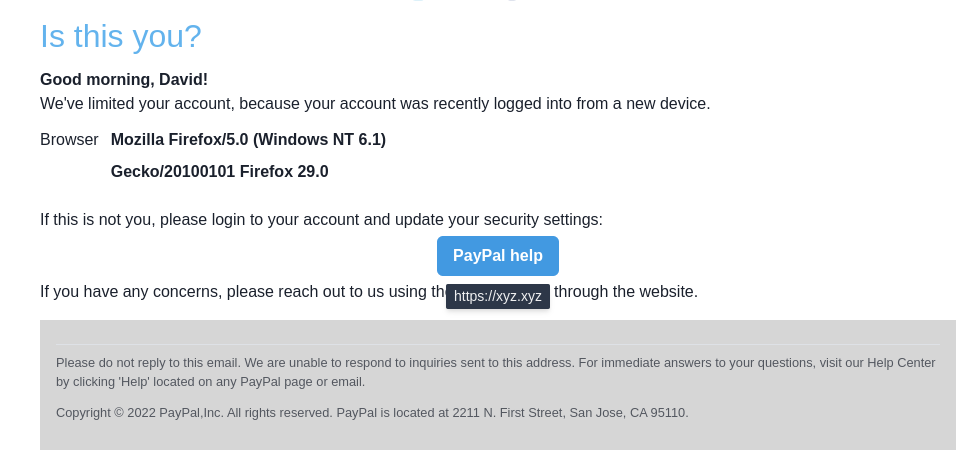
\includegraphics[width=0.48\textwidth]{figures/section2/hide_button.png}
                  \label{fig:hide-button}
              }
              \hfill
              \subfloat[The actual link is hidden behind the text]{%
                  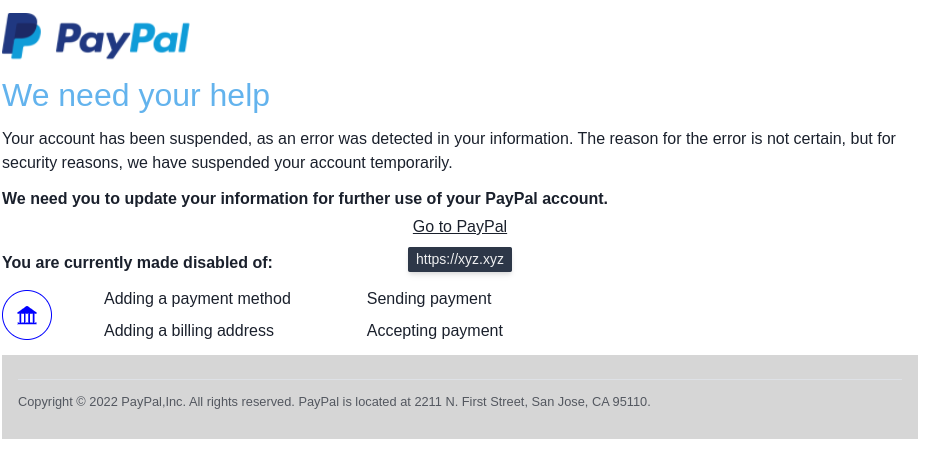
\includegraphics[width=0.48\textwidth]{figures/section2/hide_text.png}
                  \label{fig:hide-text}
              }
              \caption{Examples of hiding the actual link behind text or button}
          \end{figure}

          The primary goal of this option is to encourage the user to check for the actual destination links and not to trust the display message.

    \item \textbf{Link shortener}\\
          During our survey of phishing emails, we noticed attackers use URL shorteners to confuse the end-users. A URL shortener is a tool that creates a short, unique URL that will redirect to the specific website of the user choosing. There are multiple free URL shortening services that shorten the URL with a button click. TinyURL, Bitly, Short.io, BL.INK are some popular examples of shortening services. Table \ref{tab:shortener} shows an example of a different URL shortener. The shortened links do not expose the actual domain it redirects to. Phishers use this fact by hiding the actual domain with the help of shortening services.

          \begin{table}[!ht]
              \resizebox{\textwidth}{!}{%
                  \begin{tabular}{l p{0.8\textwidth}}
                      \hline
                      \textbf{Service} & \textbf{Shortener}                                                                              \\
                      \hline
                      Original URL     & https://www.uno.edu/academics/colaehd/ehd/elcf/educational-leadership-graduate-programs/masters \\
                      TinyURL          & https://tinyurl.com/5n6ehd6k                                                                    \\
                      bitly            & https://bit.ly/3CGFfBC                                                                          \\
                      is.gd            & https://is.gd/MKZdLO                                                                            \\
                      Tiny             & http://tiny.cc/unjpuz                                                                           \\
                      RB.GY            & https://rb.gy/nrwbqb                                                                            \\
                      \hline
                  \end{tabular} %
              }

              \caption[URL shortener examples]{Example of different URL shortener and their corresponding shortened links}
              \label{tab:shortener}
          \end{table}

          \begin{figure}[!ht]
              \centering
              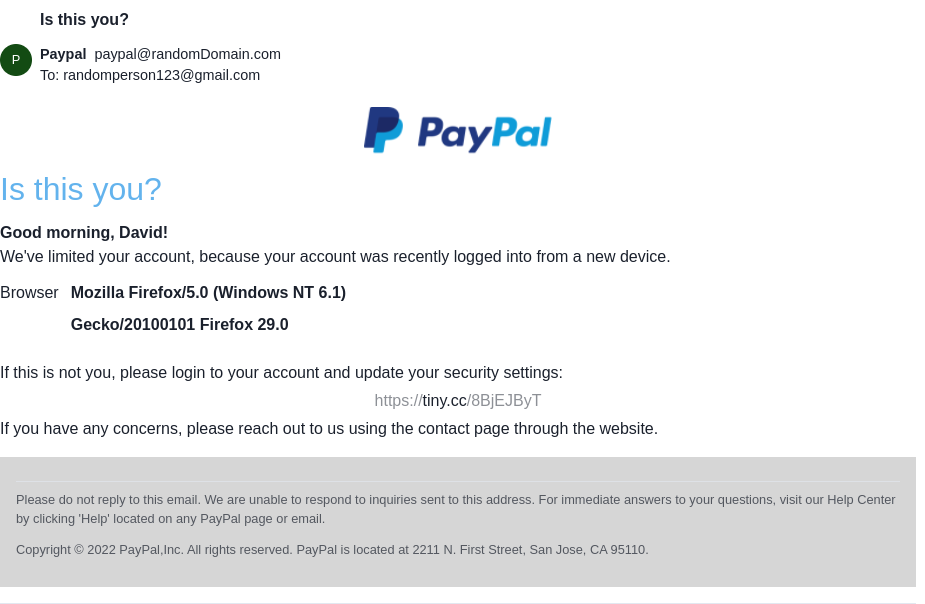
\includegraphics[width=\textwidth]{figures/section2/shortener.png}
              \caption{Example of a URL shortener option in game}
              \label{fig:shortener}
          \end{figure}

          Figure \ref{fig:shortener} shows an example of an email generated with the shortener option. The primary goal of this option is to familiarize players with different URL shortening services and how they can be used to hide actual links. In addition to just knowing how to hide links with shorteners, we want the user to know about different shortening services. Hence, every time the user chooses to hide the link with the shortening service,  we randomly choose one of the shortening services and attach a nano id \footnote{\url{https://github.com/ai/nanoid}} at the end. Table \ref{tab:shortener} shows different link shortener services included in the game with an example.


    \item \textbf{Confusion}\\
          The confusion option teaches users to be careful about familiar links that might look familiar. We focus on subdomains for this option as they are free, can be anything (including existing organization names), and can be added to any existing domains. Phishing links attempt to confuse the users by including the organization name as a subdomain.  We try to show the player this by adding "paypal" to the current domain in the game. For example, "paypal.xyz.xyz" may look like a PayPal domain but is a page in xyz.xyz.

          \begin{figure}[ht]
              \centering
              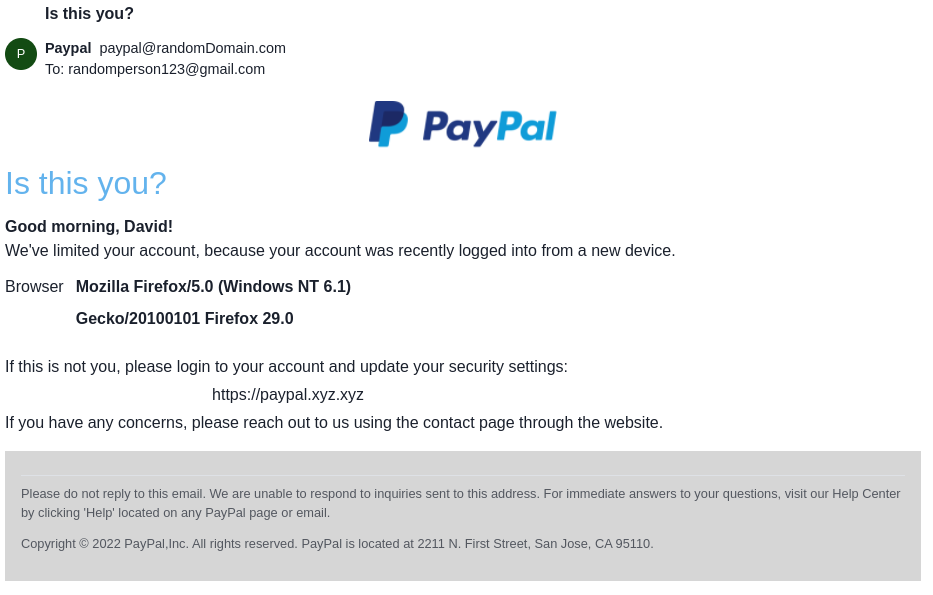
\includegraphics[width=0.9\textwidth]{figures/section2/confusion.png}
              \caption{Example of a email generated with link confusion}
              \label{fig:confusion}
          \end{figure}

    \item \textbf{Display link as is}\\
          The "display link as is" option allows players to see the actual link without modification. This option is useful when the domain purchased by the player is very similar to PayPal. For example, "paypai.com" (with i) looks similar to paypal.com. This domain can easily trick the victims into clicking the link if they are not closely paying attention. We use this option to train users on a similar-looking domain bought from the marketplace.

\end{enumerate}


Player select the link hiding method with an interactive drag and drop approach. We want the player to have immediate feedback on their action. Hence, when the player chooses an option, we immediately change the email. This visualization allows the players to see how the links are used in context to the email.

The final active skill in the game is spoofing. Existing games do not focus on training users on spoofing. However, users can easily get tricked into giving sensitive information if they receive emails from a familiar source. Various free services (Example: figure \ref{fig:spoof_sender}) send emails with custom header (custom to, reply-to, subject fields in the email) without additional verification.

\begin{figure}[ht]
    \centering
    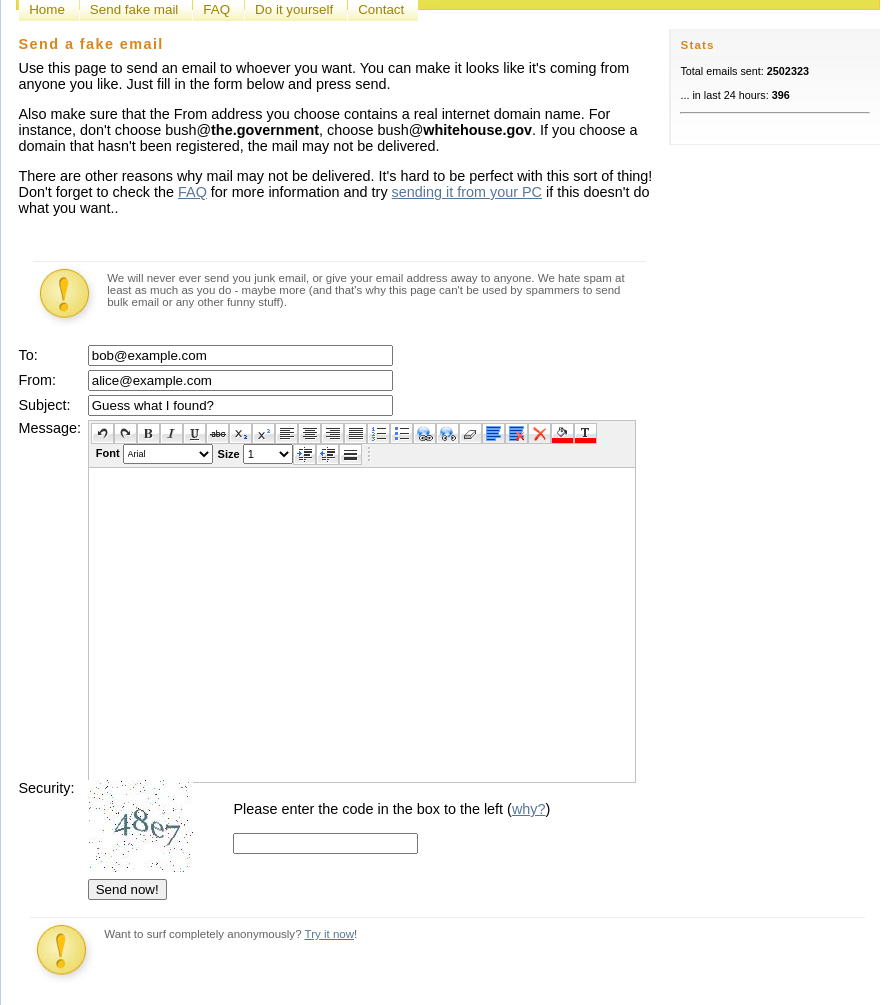
\includegraphics[width=0.6\textwidth]{figures/section2/spoof_sender.png}
    \caption[Fake email sender]{Example of a fake email sender. User can send the email to any email address as any sender.}
    \label{fig:spoof_sender}
\end{figure}

After the player unlocks the "spoof" skill, we allow the player to change the sender's email address to any valid email address. The primary goal is to show the user that the sender can be anyone, and the user has to pay attention to other details of the emails, such as context and links.

\begin{figure}[!ht]
    \centering
    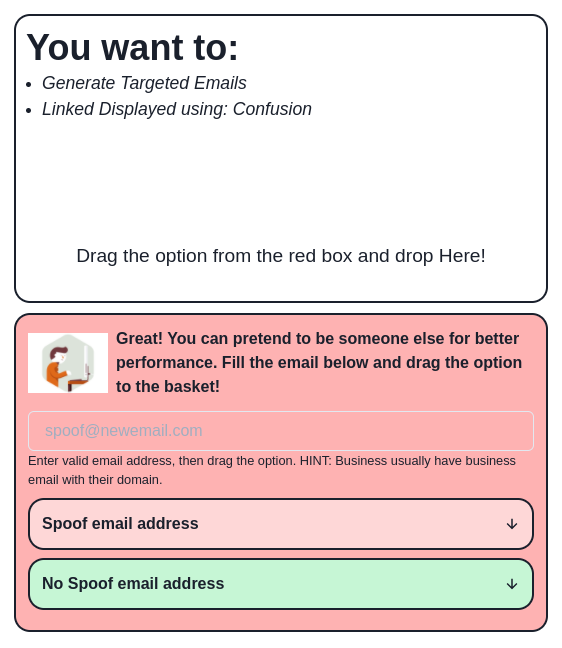
\includegraphics[width=0.4\textwidth]{figures/section2/spoofing.png}
    \caption{Spoofing option in game}
    \label{fig:spoofing}
\end{figure}

\subsection{Email efficiency}
The efficiency of the email generated by the system depends on the options chosen by the user. Each new skill can improve the efficiency of the email. We calculate the efficiency of generated email as:

\begin{center}
    \resizebox{\textwidth}{!}{
        \begin{math}
            E= \frac{\text{Sum of trained passive skill points + Sum of skill point of active skills chosen by the user}}{\text{Total Available skill points}} \times 100\%
        \end{math}
    }
\end{center}

Table \ref*{tab:efficiency} shows the max efficiency point for each skill in the game. The efficiency of passive skills is either 0 (if absent) or max efficiency points (if present), whereas active skills efficiency is calculated based on user input. Active skills options are scaled to show the efficiency of each option. For example, generating targeted (spear phishing) is more efficient as it contains personal information in emails. We add 20 points to the efficiency of the generated email if targeted to replicate this, 0 otherwise.

\begin{table}[!ht]
    \centering
    \begin{tabular}{l c}
        \hline
        Skill    & Max Efficiency Point \\
        \hline
        Spelling & 5                    \\
        Grammar  & 5                    \\
        Styling  & 10                   \\
        Research & 20                   \\
        Links    & 25                   \\
        Spoofing & 25                   \\
        \hline
    \end{tabular}%
    \caption{Efficiency of each option}
    \label{tab:efficiency}
\end{table}

Different link hiding skills have different efficiency, although close to each other. Hiding the link behind the text gives 18 points, shortening the link gives 20 points, and using confusion gives 25 points. When the player decides to display the link as is, we calculate the string similarity of the user domain with "paypal.com." If the similarity is greater than 80\%, we add 20 points to the efficiency. Else, we add 3 points to efficiency.

Similarly, for spoofing, we want to encourage players to notice that they can pretend to send the email as anyone. We compare the domain (the part after @) in the spoofed email chosen by the user with "paypal.com." Depending on similarity the similarity score, we assign points as shown in table \ref{tab:similarity_spoofed}.

\begin{table}[!ht]
    \centering
    \begin{tabular}{l c}
        \hline
        Similarity & Point \\
        \hline
        90\%       & 20    \\
        80\%       & 18    \\
        60\%       & 7     \\
        Below 60\% & 0     \\
        \hline
    \end{tabular}%
    \caption{Similarity of spoofed email domain and points assigned}
    \label{tab:similarity_spoofed}
\end{table}

We considered different keywords seen in real emails sent by organizations and wanted the players to try these keywords. For example, if the name included keywords "contact," "help," "info," "no-reply," or "noreply," we add 5 points to the efficiency. Similarly, if the email contains "paypal" in the name but was sent from a domain with a low similarity score, we add 10 points.

We calculate the efficiency based on these criteria by adding the player skill points and dividing it by the sum of all available points.

\subsection{Previous Iteration}
The initial version of the game was an open system where users could train with any skill at any given point (given they had enough amount to train). We used time to incentivize users to explore different options and generate efficient emails. The game had the same goals, options, and components but required players to avoid running out of time.

\begin{figure}[!ht]
    \centering
    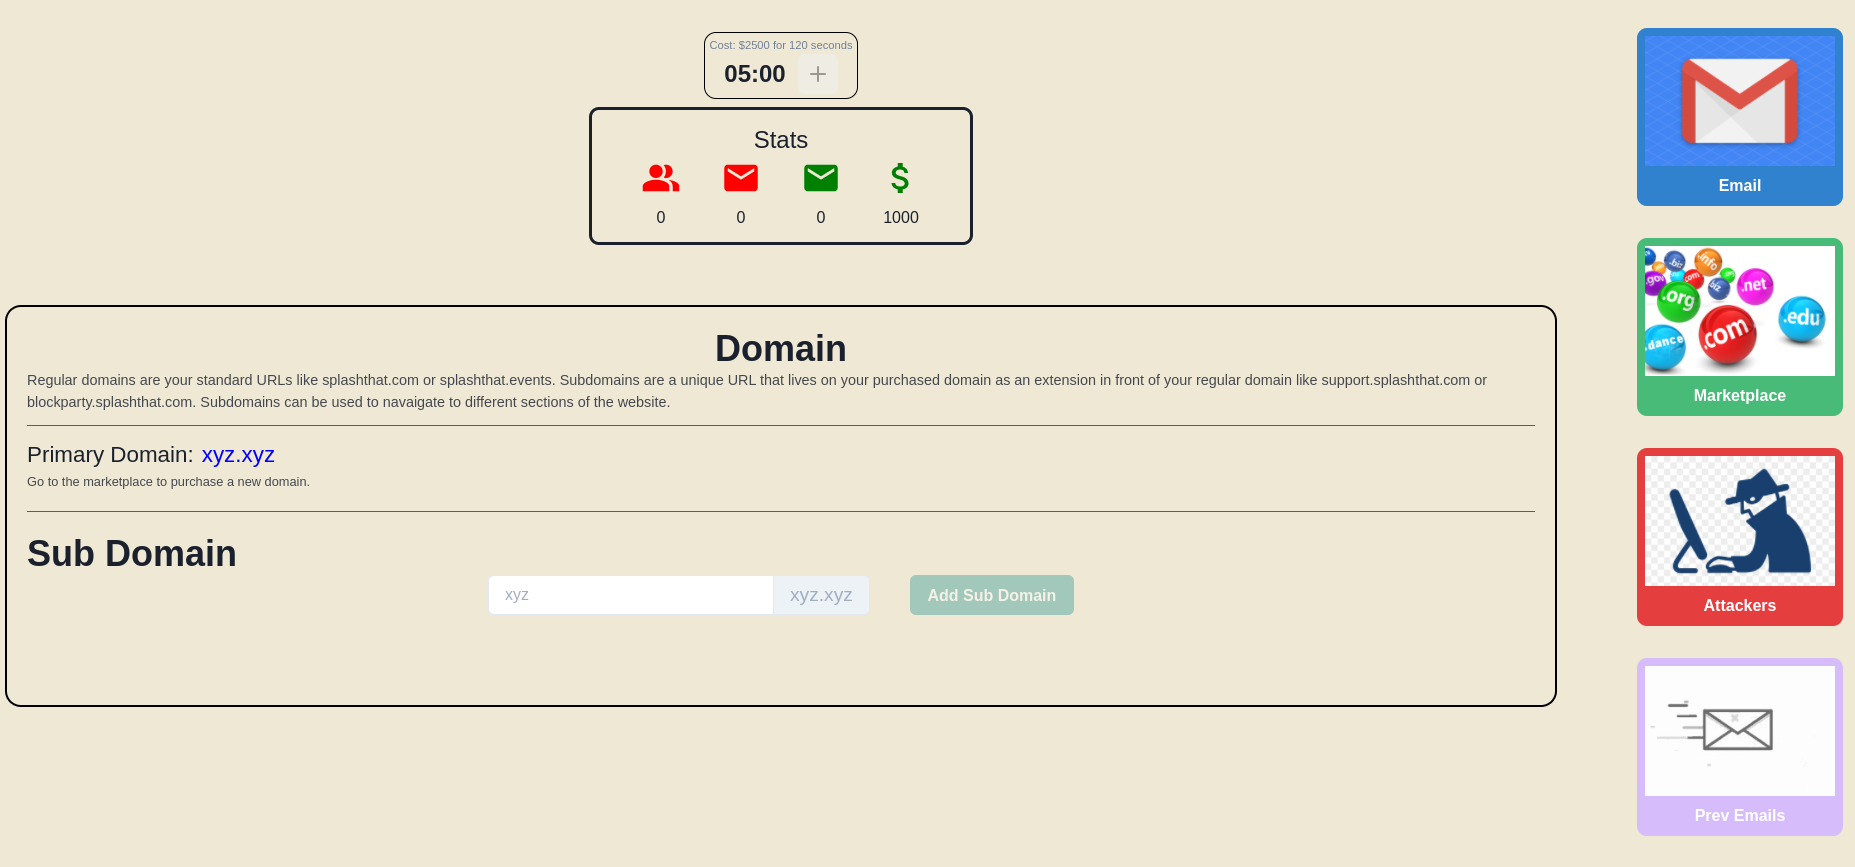
\includegraphics[width=0.9\textwidth]{figures/section2/game_initial.png}
    \caption[Initial version of the game]{Initial version of the game included timer to incentivize the user to complete the game.}
\end{figure}

We noticed a couple of drawbacks during the testing of the initial version. First, we realized that players were constantly worried about running out of time and were not reading the emails and paying attention to all the options. This limitation challenged us to balance the game such that users had enough time to read all the emails but could not brute force (send unlimited emails to achieve the goal) through it. However, different players played the game at different paces, which made us realize that time might not be the best way to incentivize the players to complete the game.

Second, we wanted to ensure that all the players had a similar experience and explored all possible training options. Unfortunately, the open system prevented us from confirming that all the players explored the training module in the same order. It also allowed the player to train on multiple modules simultaneously. Due to this, some combination of training orders allowed players to skip some training modules.

In order to ensure players were exploring all training modules and had the same experience, we developed a new system that lets the player focus on a particular skill at a time. The current design unlocks each skill in part and ensures users are familiar with current techniques before moving on to a new technique.

\subsection{Weekly Goals}
The game's current design divides the game into four parts (week). We let the player generate a limited number of emails each week. Each week unlocks new skills that the user must train on to achieve the goal. Table \ref{tab:weekly-goals} shows skills unlocked each week along with the weekly goals and number of emails they can send each week. The weekly goals are adjusted based on the efficiency of the emails for the current week. As discussed above, the user's current skills determine the efficiency of the email. We determined the weekly goal through the process of trial and error. The weekly goals increase each week as we unlock new skills, which leads to more efficient emails.

\begin{table}[ht]
    \centering
    % \resizebox{\textwidth}{!}{%
    \begin{tabular}{c l r r}
        \hline

        \textbf{Week} & \textbf{Trainable Skills}      & \textbf{Weekly Goal} & \textbf{No. of Emails} \\
        \hline
        1             & None                           & 1,500                & 5                      \\
        2             & Spelling, Grammar, Links       & 15,000               & 10                     \\
        3             & Marketplace, Styling, Research & 38,000               & 10                     \\
        4             & Spoofing                       & 80,000               & 10                     \\
        \hline
    \end{tabular}%
    % }
    \caption{Different week with their corresponding skills and goals}
    \label{tab:weekly-goals}
\end{table}

Week 1 does not contain any trainable skill and solely focuses on language in the email. We want the player to know that low-tier phishing emails may contain spelling and grammar problems, whereas official/legitimate emails are usually proofread and do not contain these issues.

Week 2 lets the user train on spelling, grammar, and links. Players can remove spelling and grammar errors by training language skills and entirely focus on different link hiding techniques. We let the players play with the link skill by giving a higher number of emails for the week.

Week 3 opens the marketplace along with styling and research. At this point, users have explored different ways to hide the link, and we want to focus on links that might look similar to trick the user. To force users to explore different domains, we disable all link hiding techniques and force users to show the link as is. This forces the player to utilize the marketplace and explore multiple domains.

Finally, week 4 disables the marketplace and unlocks spoofing. We unlock the link hiding skill and let the user play around with all the options. Our initial survey showed players only required half the available emails to figure out spoofing. However, we want the player to play around with all possible combinations for the final few emails, due to which we have a higher number of emails to send than required.